\documentclass[../AnalisideiRequisiti.tex]{subfiles}

\begin{document}
	% Il comando UserCase accetta primo una label nel caso serva un link verso di lui \refer{label} poi 
	% attore primario
	% attore secondario
	% Descrizione
	% Precondi
	% Post
	% Scenario principale
	% Scenari alternativi 

	\chapter{Casi d'uso}
	\section{Descrizione}
	I \glossario{casi d'uso}{caso d'uso} verranno identificati nel seguente modo: 
	
	\begin{center}
		UC[Codice padre]*.[Codice identificativo]
	\end{center}
	
	\begin{itemize}
		\item \textbf{Codice padre:} identifica il codice del caso d'uso da cui è stato generato il caso d'uso identificato, se non esiste il campo va tralasciato;
		\item \textbf{Codice identificativo:} identifica il caso d'uso univocamente.
	\end{itemize}
	
	\noindent Ogni caso d'uso è inoltre definito secondo la seguente struttura:
	\begin{itemize}
		\item \textbf{Attore Principale:} indica gli attori principali (ad esempio l'utente generico) del caso d'uso;
		\item \textbf{Attore Secondario:} indica gli attori secondari (ad esempio entità di autenticazione esterne) del caso d'uso;
		\item \textbf{Descrizione:} riporta una breve descrizione del caso d'uso;
		\item \textbf{Precondizione:} specifica le condizioni che sono identificate come vere prima del verificarsi degli eventi del caso d'uso;
		\item \textbf{Postcondizione:} specifica le condizioni che sono identificate come vere dopo il verificarsi degli eventi del caso d'uso;
		\item \textbf{Scenario Principale:} descrive il flusso degli eventi, a volte attraverso l'uso di una lista numerata o non, specificando i casi d'uso generati;
		\item \textbf{Scenari Alternativi:} specifica casi di errore o eventi non previsti nello scenario principale;
		
	\end{itemize}

	\section{UC0:Avvio Applicazione}
	\begin{figure}[H]
		\caption{UC0}
		\centering
		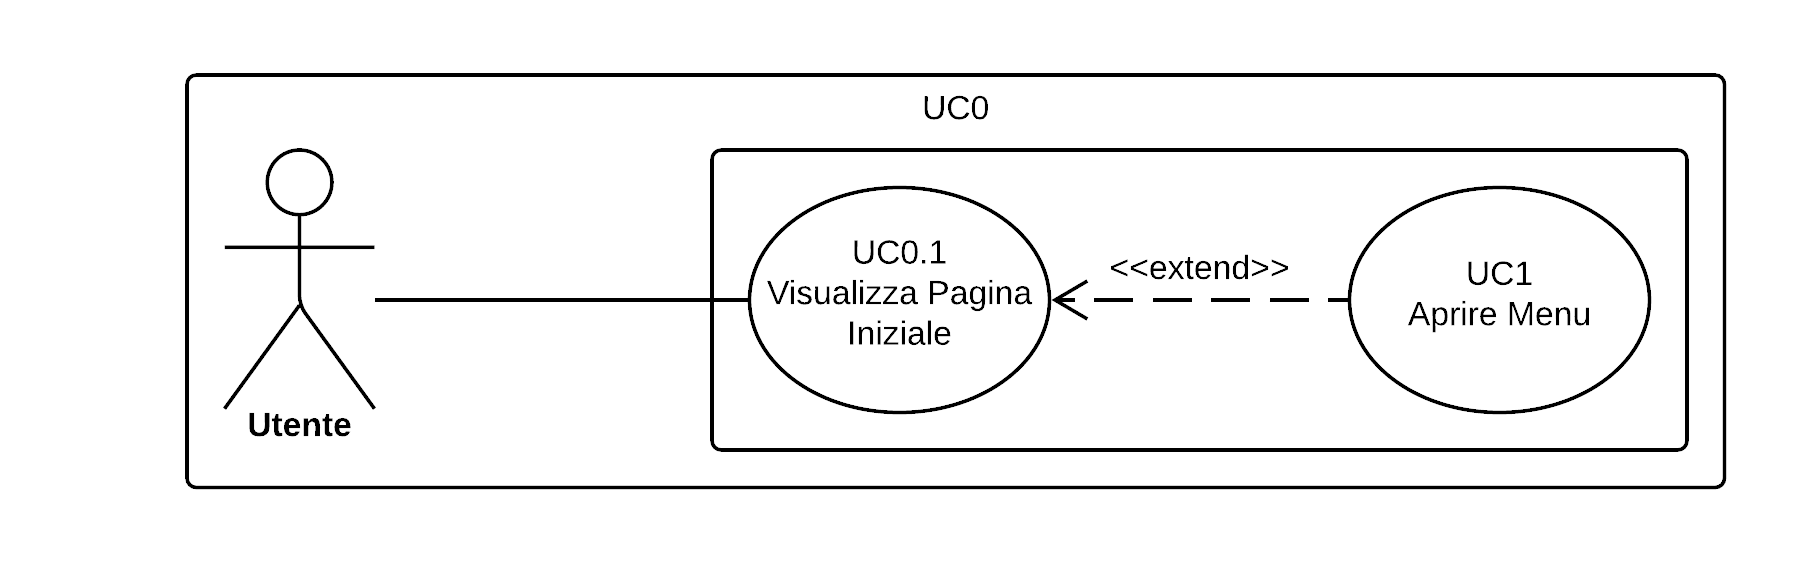
\includegraphics[width=\textwidth]{../img/UC00.png}
	\end{figure}
	\UserCase
	{UC0}
	{Utente}
	{Non previsto}
	{L'attore avvia l'applicazione DeSpeect}
	{Il software Despeect è correttamente installato}
	{Il programma è correttamente avviato}
	{Viene visualizzata la pagina iniziale \refer{UC0.1}}
	{Non previsti}
	
	\section{UC0.1:Visualizza Pagina Iniziale}
	\UserCase
	{UC0.1}
	{Utente}
	{Non previsto}
	{L'attore visualizza la pagina iniziale}
	{Il software Despeect è correttamente avviato \refer{UC0}}
	{Il programma visualizza la pagina iniziale}
	{L'attore può caricare un file Json aprendo il menu \refer{UC1}}
	{Non previsti}
	
	\section{UC1:Aprire Menu}
	\begin{figure}[H]
	\caption{UC1}
	\centering
	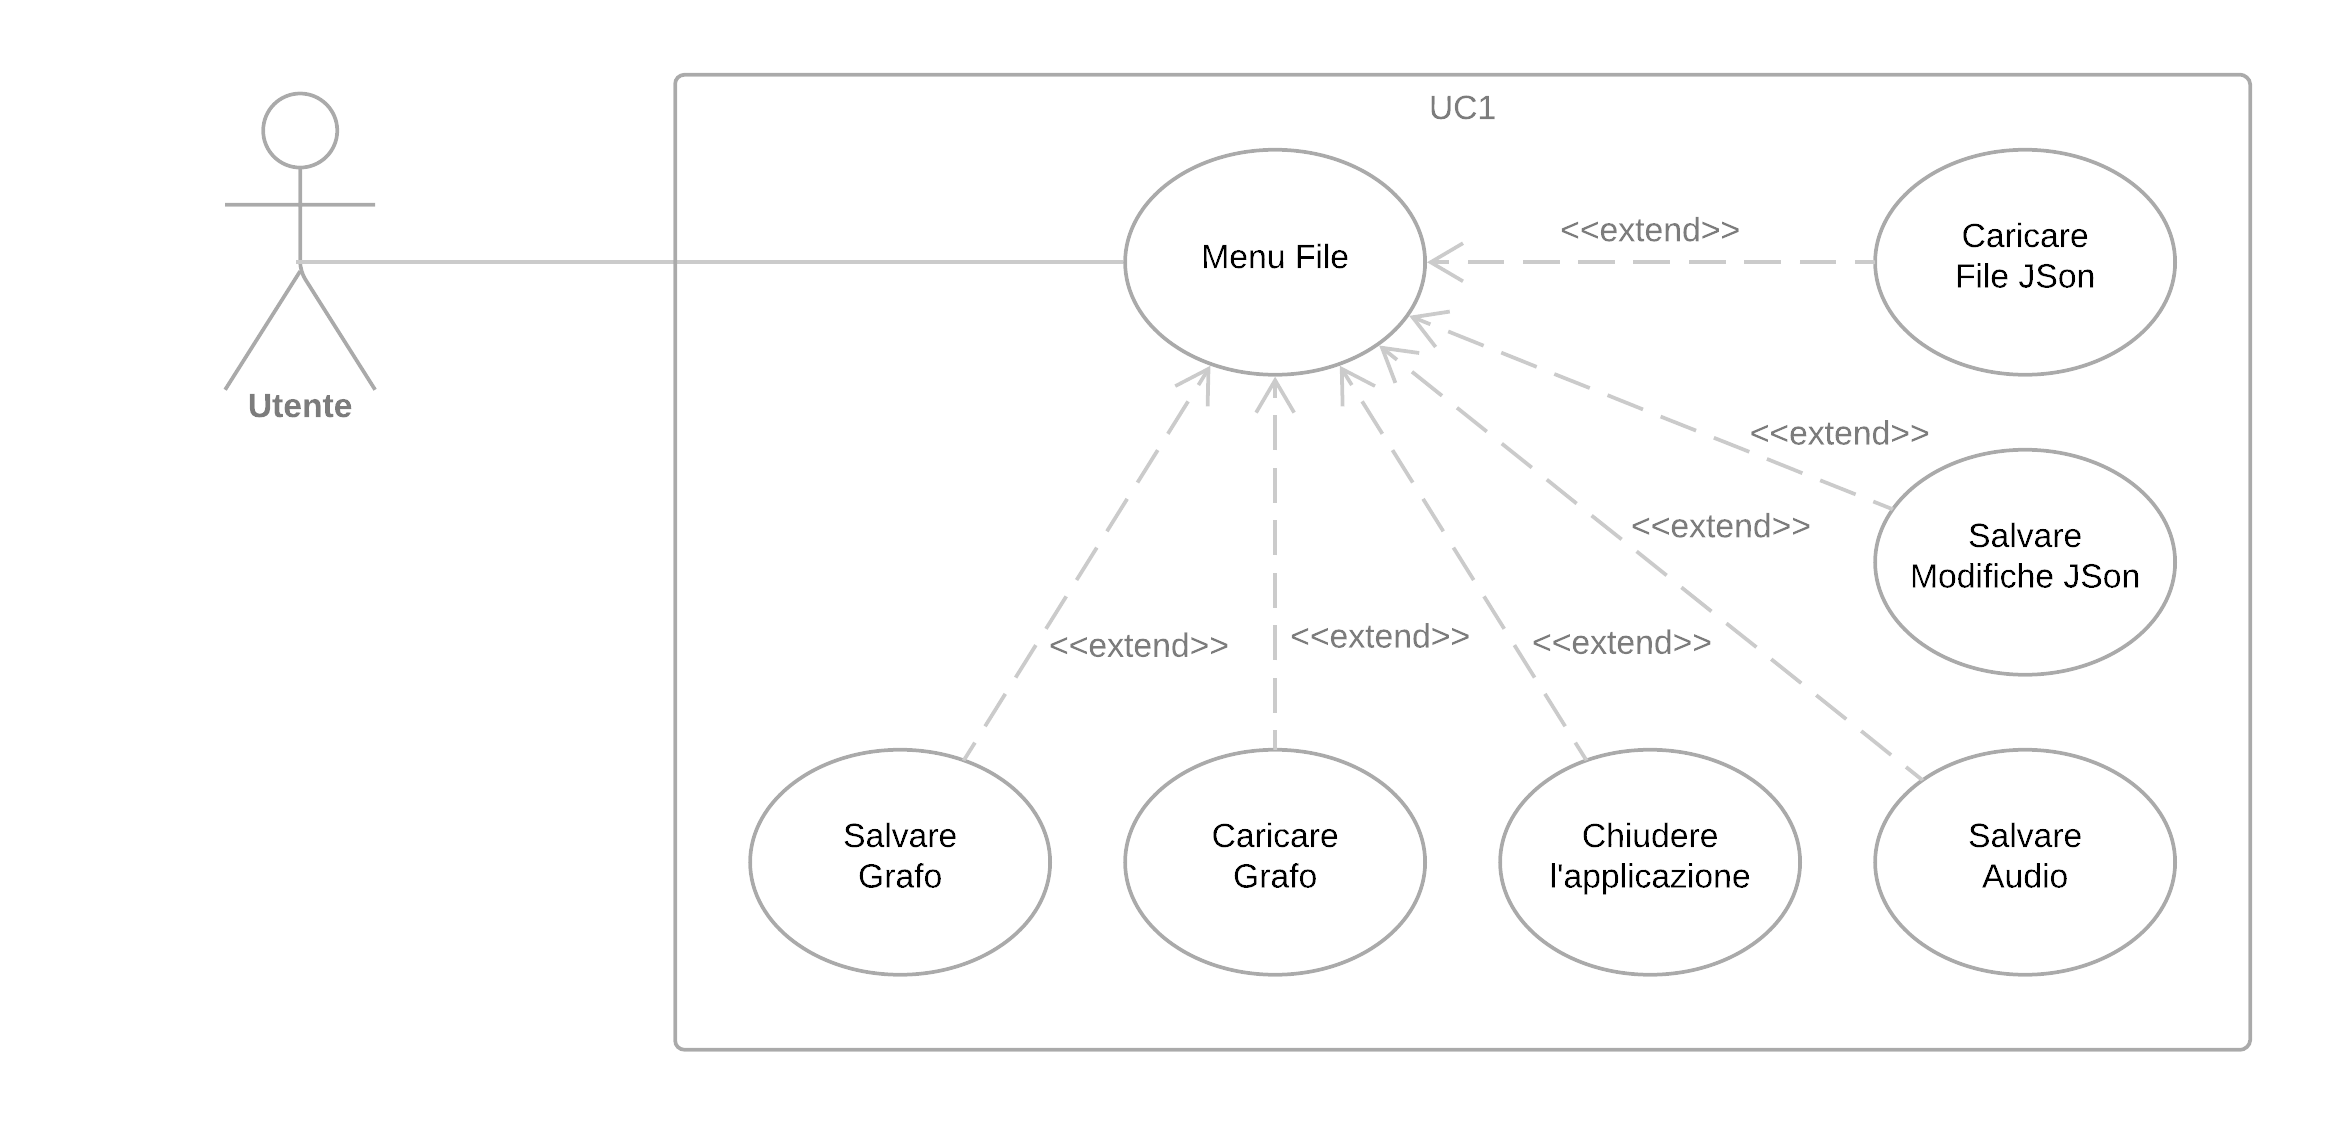
\includegraphics[width=\textwidth]{../img/UC01.png}
	\end{figure}
	\UserCase
	{UC1}
	{Utente}
	{Non previsto}
	{L'attore vuole visualizzare il menu}
	{Il programma visualizza la pagina iniziale \refer{UC0.1}}
	{Viene selezionata una voce del menu o cambiato il focus}
	{	\begin{enumerate}
			\item{} L'attore preme sul menu
			\item{} Il menu si apre e offre le seguenti scelte:
		\begin{itemize}
		\item{} L'attore può caricare un file JSon \refer{UC2}
		\item{} L'attore può salvare le modifiche al file JSon \refer{UC11}
		\item{} L'attore può salvare l'audio prodotto da Speect \refer{UC4}
		\item{} L'attore può chiudere l'applicazione \refer{UC5}
		\item{} L'attore può caricare un grafo \refer{UC8}
		\item{} L'attore può salvare un grafo \refer{UC9}
		\end{itemize}
	\end{enumerate}
	}
	{Non previsti}

	\section{UC2:Caricamento JSon}
	\begin{figure}[H]
		\caption{UC2}
		\centering
		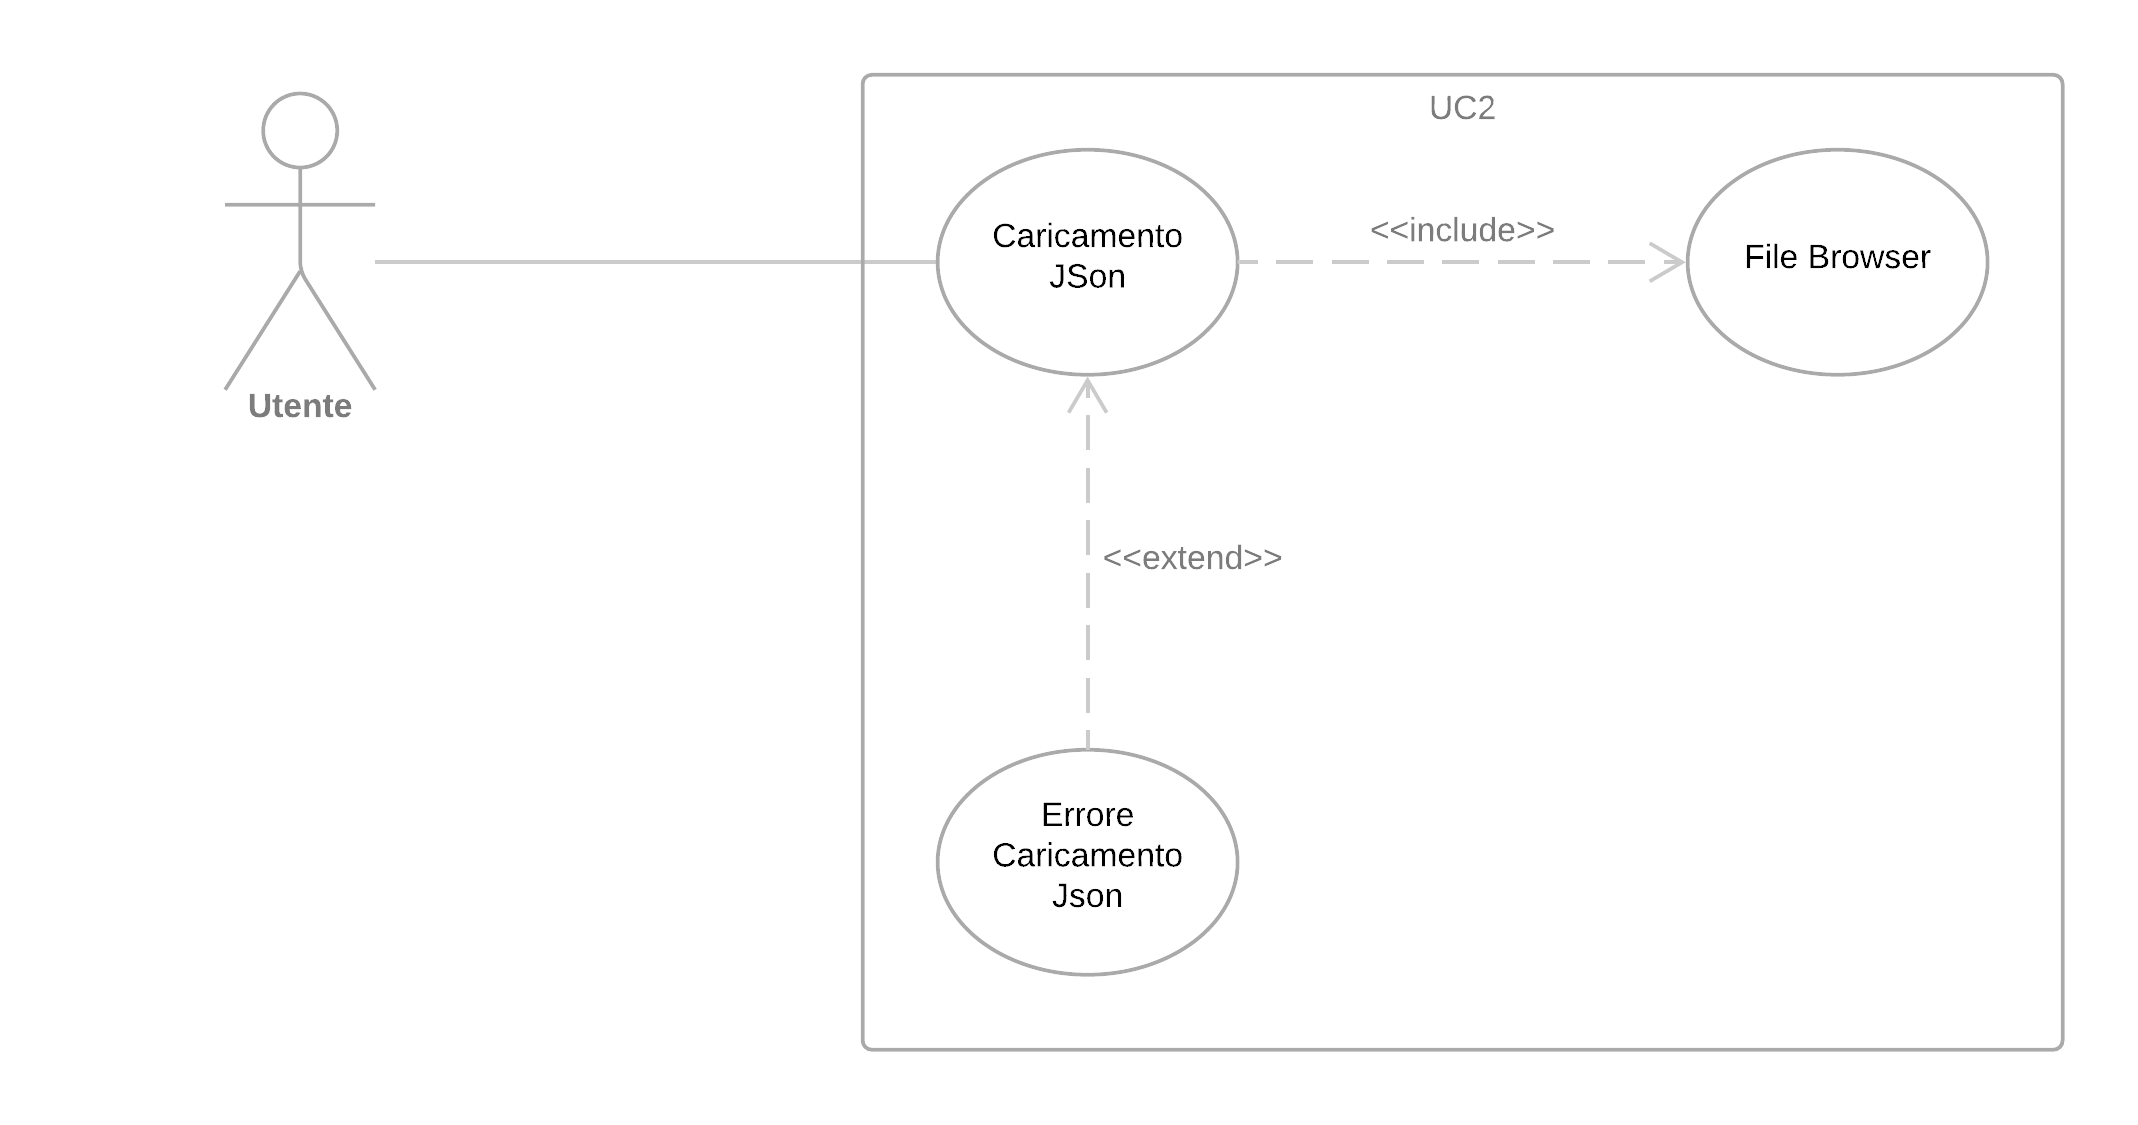
\includegraphics[width=\textwidth]{../img/UC02.png}
	\end{figure}
	\UserCase
	{UC2}
	{Utente}
	{Non previsto}
	{L'attore vuole caricare un file JSon}
	{L'attore ha selezionato la voce nel menu \refer{UC1}}
	{Viene inizializzato Speect con il file JSon selezionato e aggiornata la GUI}
	{
		\begin{itemize}
			\item{} Viene aperto il file browser per caricare \refer{UC3}
			\item{} L'attore seleziona il file tramite il file browser
			\item{} L'attore preme Carica
			\item{} Il file viene dato a Speect che prova l'inizializzazione
			\item{} Viene visualizzato il percorso del file nella apposito spazio \ref{fig:GUI}
		\end{itemize}
	}
	{Speect fallisce l'inizializzazione e l'attore visualizza il messaggio del errore relativo al file \refer{UC2.1}}
	\section{UC2.1:Errore Caricamento JSon}
	\UserCase
	{UC2.1}
	{Utente}
	{Non previsto}
	{Durante l'inizializzazione Speect fallisce ritornando un errore }
	{L'attore carica un file JSon non corretto}
	{L'errore è visualizzato a schermo e viene ripristinato lo stato precedente e ridato controllo all'attore}
	{Avvenimento dell'errore in fase di caricamento}
	{Non previsti}

	\section{UC3:File Browser analizzare QFileDialog (parlare con Marco perchè manco io capisco bene) va sistemato tutto il 3}
	\begin{figure}[H]
		\caption{UC3}
		\centering
		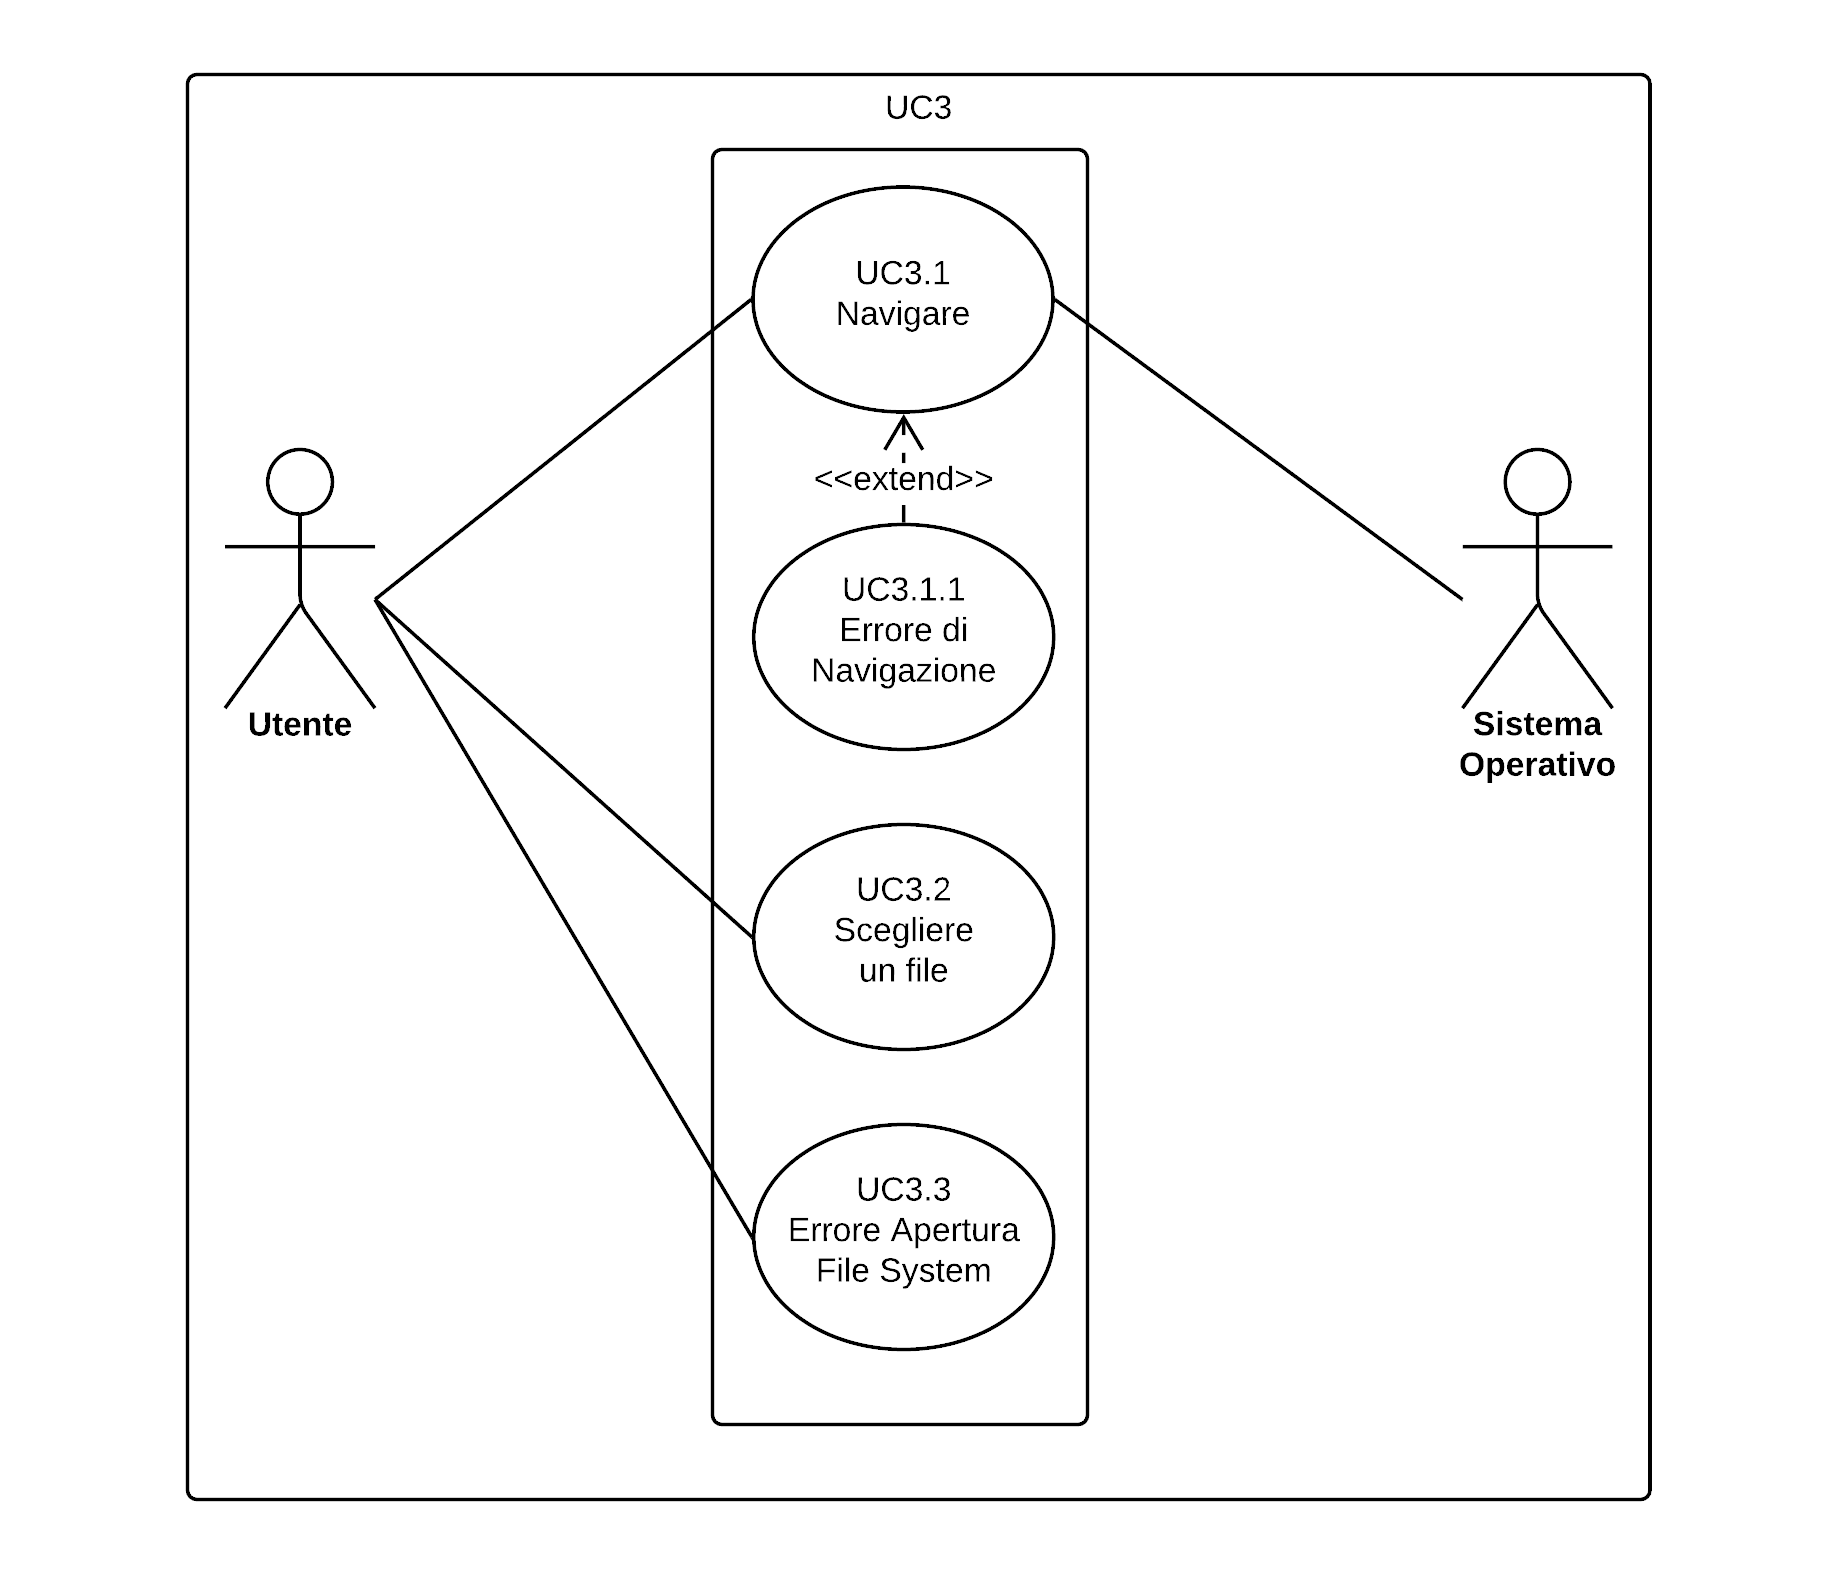
\includegraphics[width=\textwidth]{../img/UC03.png}
	\end{figure}
	\UserCase
	{UC3}
	{Utente}
	{Sistema Operativo}
	{L'attore deve navigare nel file system alla ricerca di un file o di una cartella}
	{L'attore deve selezionare un file o raggiungere una cartella}
	{Viene selezionato il file da caricare o la cartella in cui salvare}
	{
		\begin{itemize}
			\item{} Il file browser viene visualizzato dall'attore
			\item{} L'attore naviga nel file \glossario{file system}{file system} cercando il suo file \refer{UC3.1}
			\item{} L'attore seleziona un file \refer{UC3.2}
		\end{itemize}
	}
	{Fallisce la richiesta di apertura del file browsing del SO corrente}
	\section{UC3.1:Navigazione}
	\UserCase
	{UC3.1}
	{Utente}
	{Non previsto}
	{L'attore vuole navigare nel suo file system}
	{Il file \glossario{browser}{browser} è aperto}
	{E' possibile navigare nel file system}
	{
		\begin{itemize}
			\item{} L'attore può aprire cartelle \refer{UC3.1.1}
			\item{} L'attore può creare nuove cartelle \refer{UC3.1.2}
			\item{} L'attore può tornare alla cartella padre \refer{UC3.1.3}
		\end{itemize}
	}
	{Non previsti}	
	\section{UC3.1.1:Aprire cartelle}
	\UserCase
	{UC3.1.1}
	{Utente}
	{Non previsto}
	{L'attore vuole aprire una cartella e ha i permessi per farlo}
	{Il file browser visualizza la cartella}
	{Viene aperta la cartella e visualizzato il suo contenuto}
	{
		\begin{itemize}
			\item{} L'attore fa un doppio click sulla cartella
			\item{} La cartella viene aperta
			\item{} L'attore visualizza il contenuto della cartella
		\end{itemize}
	}
	{L'attore non ha i permessi necessari, viene visualizzato l'errore di navigazione \refer{UC3.3}}
	\section{UC3.1.2:Creare cartelle}
	\UserCase
	{UC3.1.2}
	{Utente}
	{Non previsto}
	{L'attore vuole creare una cartella}
	{L'attore ha i permessi per creare una cartella}
	{Viene creata una cartella}
	{
		\begin{itemize}
		\item{} L'attore preme il tasto per creare la cartella
		\item{} La cartella viene creata
		\item{} L'attore visualizza la nuova cartella
		\end{itemize}
	}
	{L'attore non ha i permessi necessari, viene visualizzato l'errore di navigazione \refer{UC3.3}}

	\section{UC3.1.3:Ritorno alla cartella Padre}
\UserCase
{UC3.1.3}
{Utente}
{Non previsto}
{L'attore preme sul tasto per tornare alla cartella padre}
{Esiste una cartella padre}
{Viene visualizzato il contenuto della cartella padre}
{L'attore ritorna alla cartella padre}
{L'attore non ha i permessi necessari, viene visualizzato l'errore di navigazione \refer{UC3.3}}
	\section{UC3.2:Scegliere un file}
\UserCase
{UC3.2}
{Utente}
{Non previsto}
{L'attore seleziona un file}
{Il file browser è aperto correttamente}
{Il file scelto viene evidenziato}
{
	\begin{itemize}
		\item{} L'attore clicca sull' elemento
		\item{} L'elemento selezionato viene evidenziato
	\end{itemize}
}
{Non previsti}
\section{UC3.3:Errore di Navigazione}
\UserCase
{UC3.3}
{Utente}
{Non previsto}
{L'attore cerca di fare un operazione senza i permessi necessari}
{L'attore ha cercato di effettuare un operazione senza i permessi necessari}
{Viene visualizzato l'errore e nessuna operazione viene svolta}
{Avvenimento dell'errore in fase di navigazione}
{Non previsti}

\section{UC4:Salvataggio Audio Prodotto}
\begin{figure}[H]
	\caption{UC4}
	\centering
	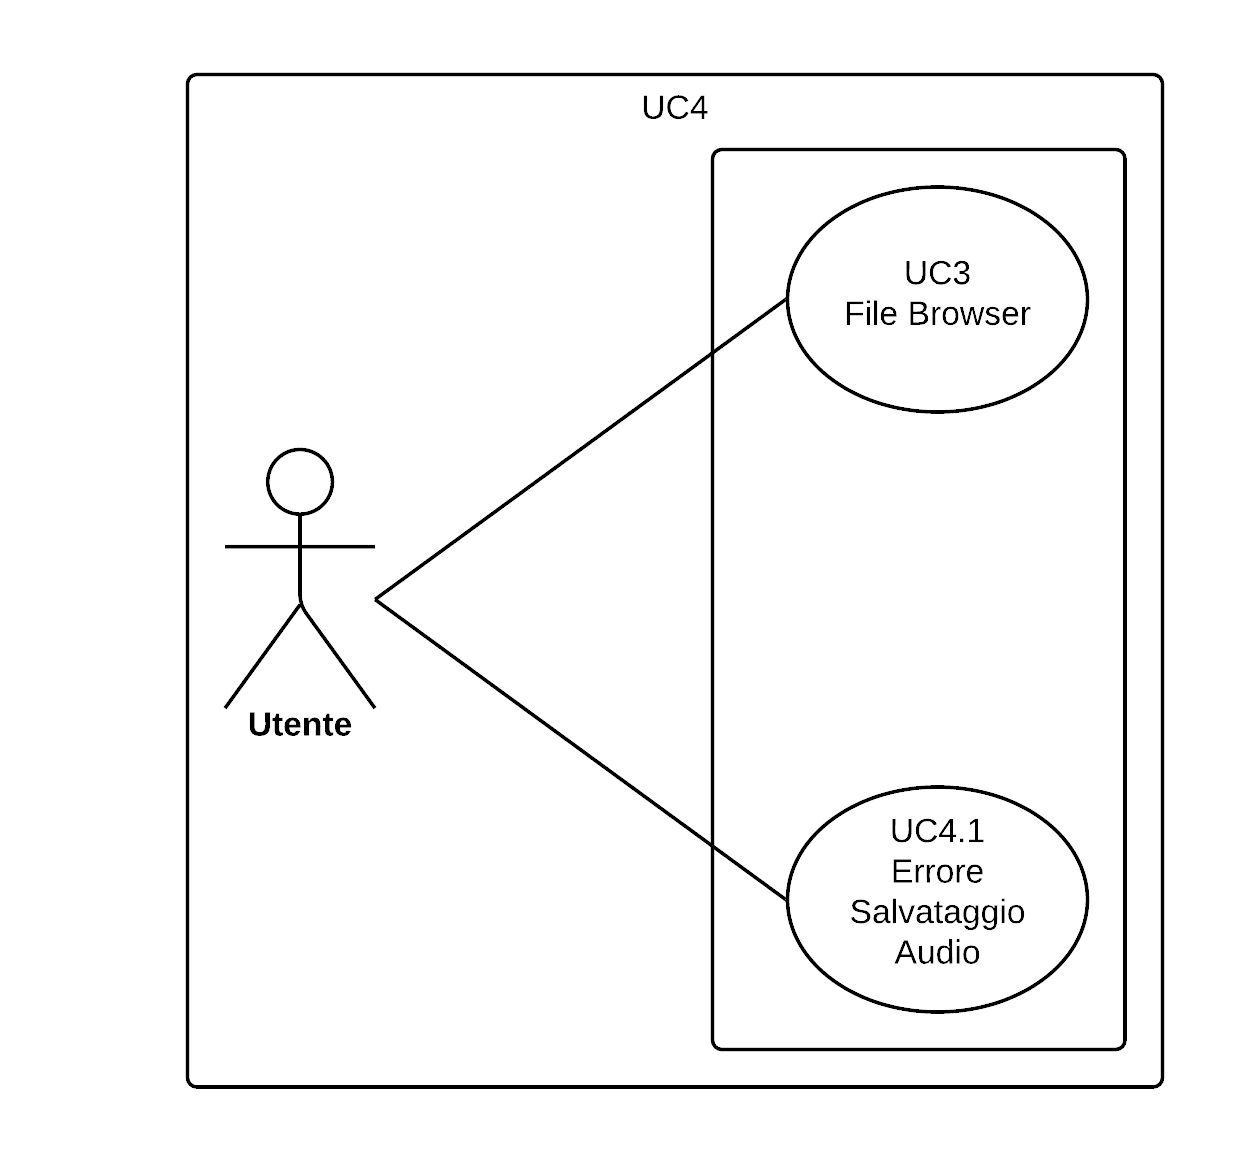
\includegraphics[width=\textwidth]{../img/UC04.png}
\end{figure}
\UserCase
{UC4}
{Utente}
{Non previsto}
{L'attore vuole salvare l'audio}
{Speect è inizializzato \refer{UC2}}
{L'audio è salvato in un file}
{
		\begin{itemize}
		\item{} Viene aperto il file browser per il salvataggio \refer{UC3}
		\item{} L'attore seleziona la cartella di destinazione tramite il file browser 
		\item{} L'attore scrive il nome del file nella barra di testo
		\item{} L'attore preme su Salva 
		\item{} Speect compila producendo il file desiderato o un errore  \refer{UC4.1}
		\item{} Se non è avvenuto un errore il file viene salvato nella destinazione con estensione .WAV
		\end{itemize}
}
{L'attore visualizza un messaggio di errore \refer{UC4.1}}		
\section{UC4.1:Errore Salvataggio Audio}
\UserCase
{UC4.1}
{Utente}
{Non previsto}
{Avviene un errore durante il salvataggio dell'audio}
{L'attore ha cercato di salvare un file audio}
{Viene visualizzato l'errore e nessuna operazione viene eseguita}
{Avvenimento dell'errore in fase di salvataggio}
{Non previsti}

\section{UC5:Uscita Applicazione}
\begin{figure}[H]
	\caption{UC5}
	\centering
	
\includegraphics[width=\textwidth]{../img/UC05.png}
\end{figure}
\UserCase
{UC5}
{Utente}
{Non previsto}
{L'attore vuole chiudere l'applicazione}
{Viene confermata la chiusura dell'applicazione}
{L'applicazione viene terminata}
{Chiusura dell'applicazione}
{L'attore annulla la chiusura dell'applicazione}

\section{UC5.1:Chiusura Interfaccia Grafica}
\UserCase
{UC5.1}
{Utente}
{Non previsto}
{L'attore visualizza un finestra di conferma}
{L'applicazione è in esecuzione}
{L'attore conferma o annulla la chiusura dell'applicazione}
{L'attore richiede la chiusura dell'applicazione}
{Non previsti}

\section{UC6:Selezione Utterance}
\begin{figure}[H]
	\caption{UC6}
	\centering
	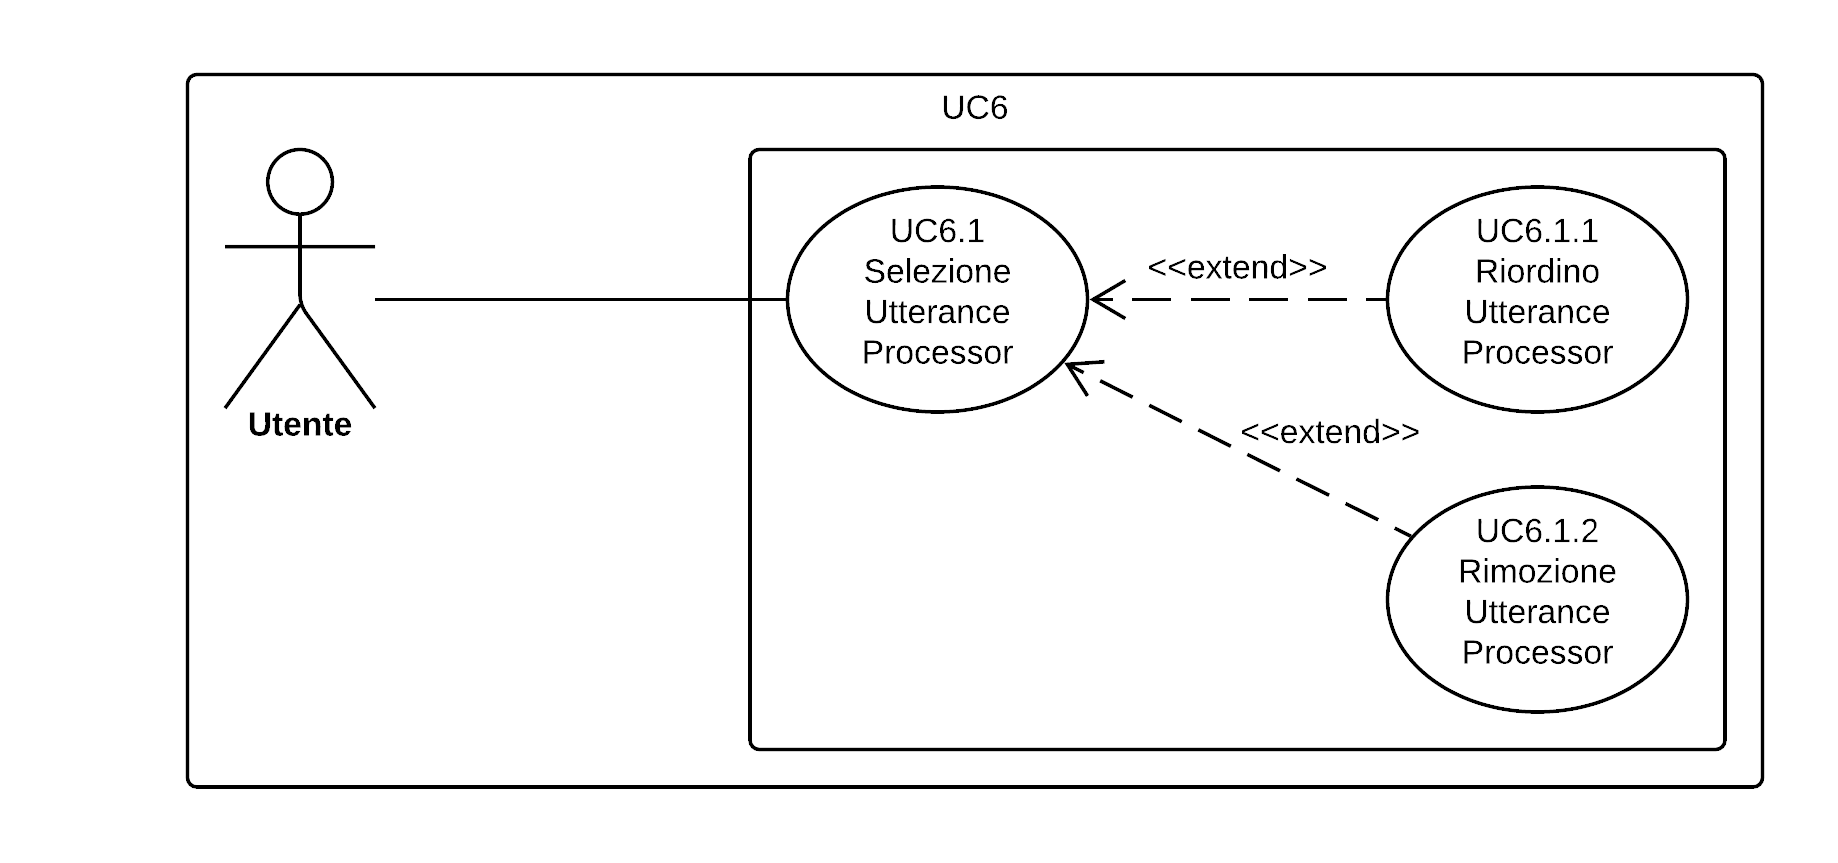
\includegraphics[width=\textwidth]{../img/UC06.png}
\end{figure}
\UserCase
{UC6}
{Utente}
{Non previsto}
{L'attore vuole selezionare la Utterance desiderata}
{Un file JSon è stato caricato (\refer{UC2}) correttamente }
{Vengono mostrati gli Utterance Processors utilizzati da Speect per tale Utterance type}
{
	\begin{itemize}
		\item{} L'attore clicca sul menu a tendina
		\item{} Viene aperto il menu a tendina
		\item{} L'attore clicca sul Utterance type desiderata
		\item{} Vengono mostrati a schermo i nomi degli Utterance Processor utilizzati negli appositi spazi \ref{fig:GUI}		
	\end{itemize}
}
{Non previsti}

\section{UC6.1:Selezione Utterance Processor}
\UserCase
{UC6.1}
{Utente}
{Non previsto}
{L'attore vuole selezionare un Utterance Processor per spostarlo}
{Un file JSon è stato caricato correttamente \refer{UC2}}
{Vengono visualizzati i bottoni per modificare tale Utterance Processor}
{
	\begin{itemize}
		\item{} L'attore clicca sul nome dell'Utterance Processor
		\item{} Vengono visualizzati due bottoni che permettono lo spostamento grafico del Utterance Processor \refer{UC6.1.1} e un bottone che ne permette la rimozione \refer{UC6.1.2} 		
	\end{itemize}
}
{Non previsti}

\section{UC6.1.1:Riordino Utterance Processor}
\UserCase
{UC6.1.1}
{Utente}
{Non previsto}
{L'attore vuole cambiare l'ordine degli Utterance Processor}
{Un file JSon è stato caricato \refer{UC2} correttamente }
{Il file JSon viene aggiornato}
{
	\begin{itemize}
		\item{} L'attore clicca sull'Utterance Processor \refer{UC6.1}
		\item{} L'attore riordina tramite i pulsanti forniti	
		\item{} Le operazioni vengono eseguite
		\item{} Se esisteva un grafo, esso non viene modificato
		
	\end{itemize}
}
{Non previsti}

\section{UC6.1.2:Rimozione Utterance Processor}
\UserCase
{UC6.1.2}
{Utente}
{Non previsto}
{L'attore vuole rimuovere un Utterance Processor}
{Un file JSon è stato caricato \refer{UC2} correttamente }
{Il file JSon viene aggiornato}
{
	\begin{itemize}
		\item{} L'attore clicca sull'Utterance Processor \refer{UC6.1}
		\item{} L'attore rimuove tramite il pulsante fornito	
		\item{} L'operazione viene eseguita
		\item{} Se esisteva un grafo, esso non viene modificato
		
	\end{itemize}
}
{Non previsti}

\section{UC7:Esecuzione}
\begin{figure}[H]
	\caption{UC7}
	\centering
	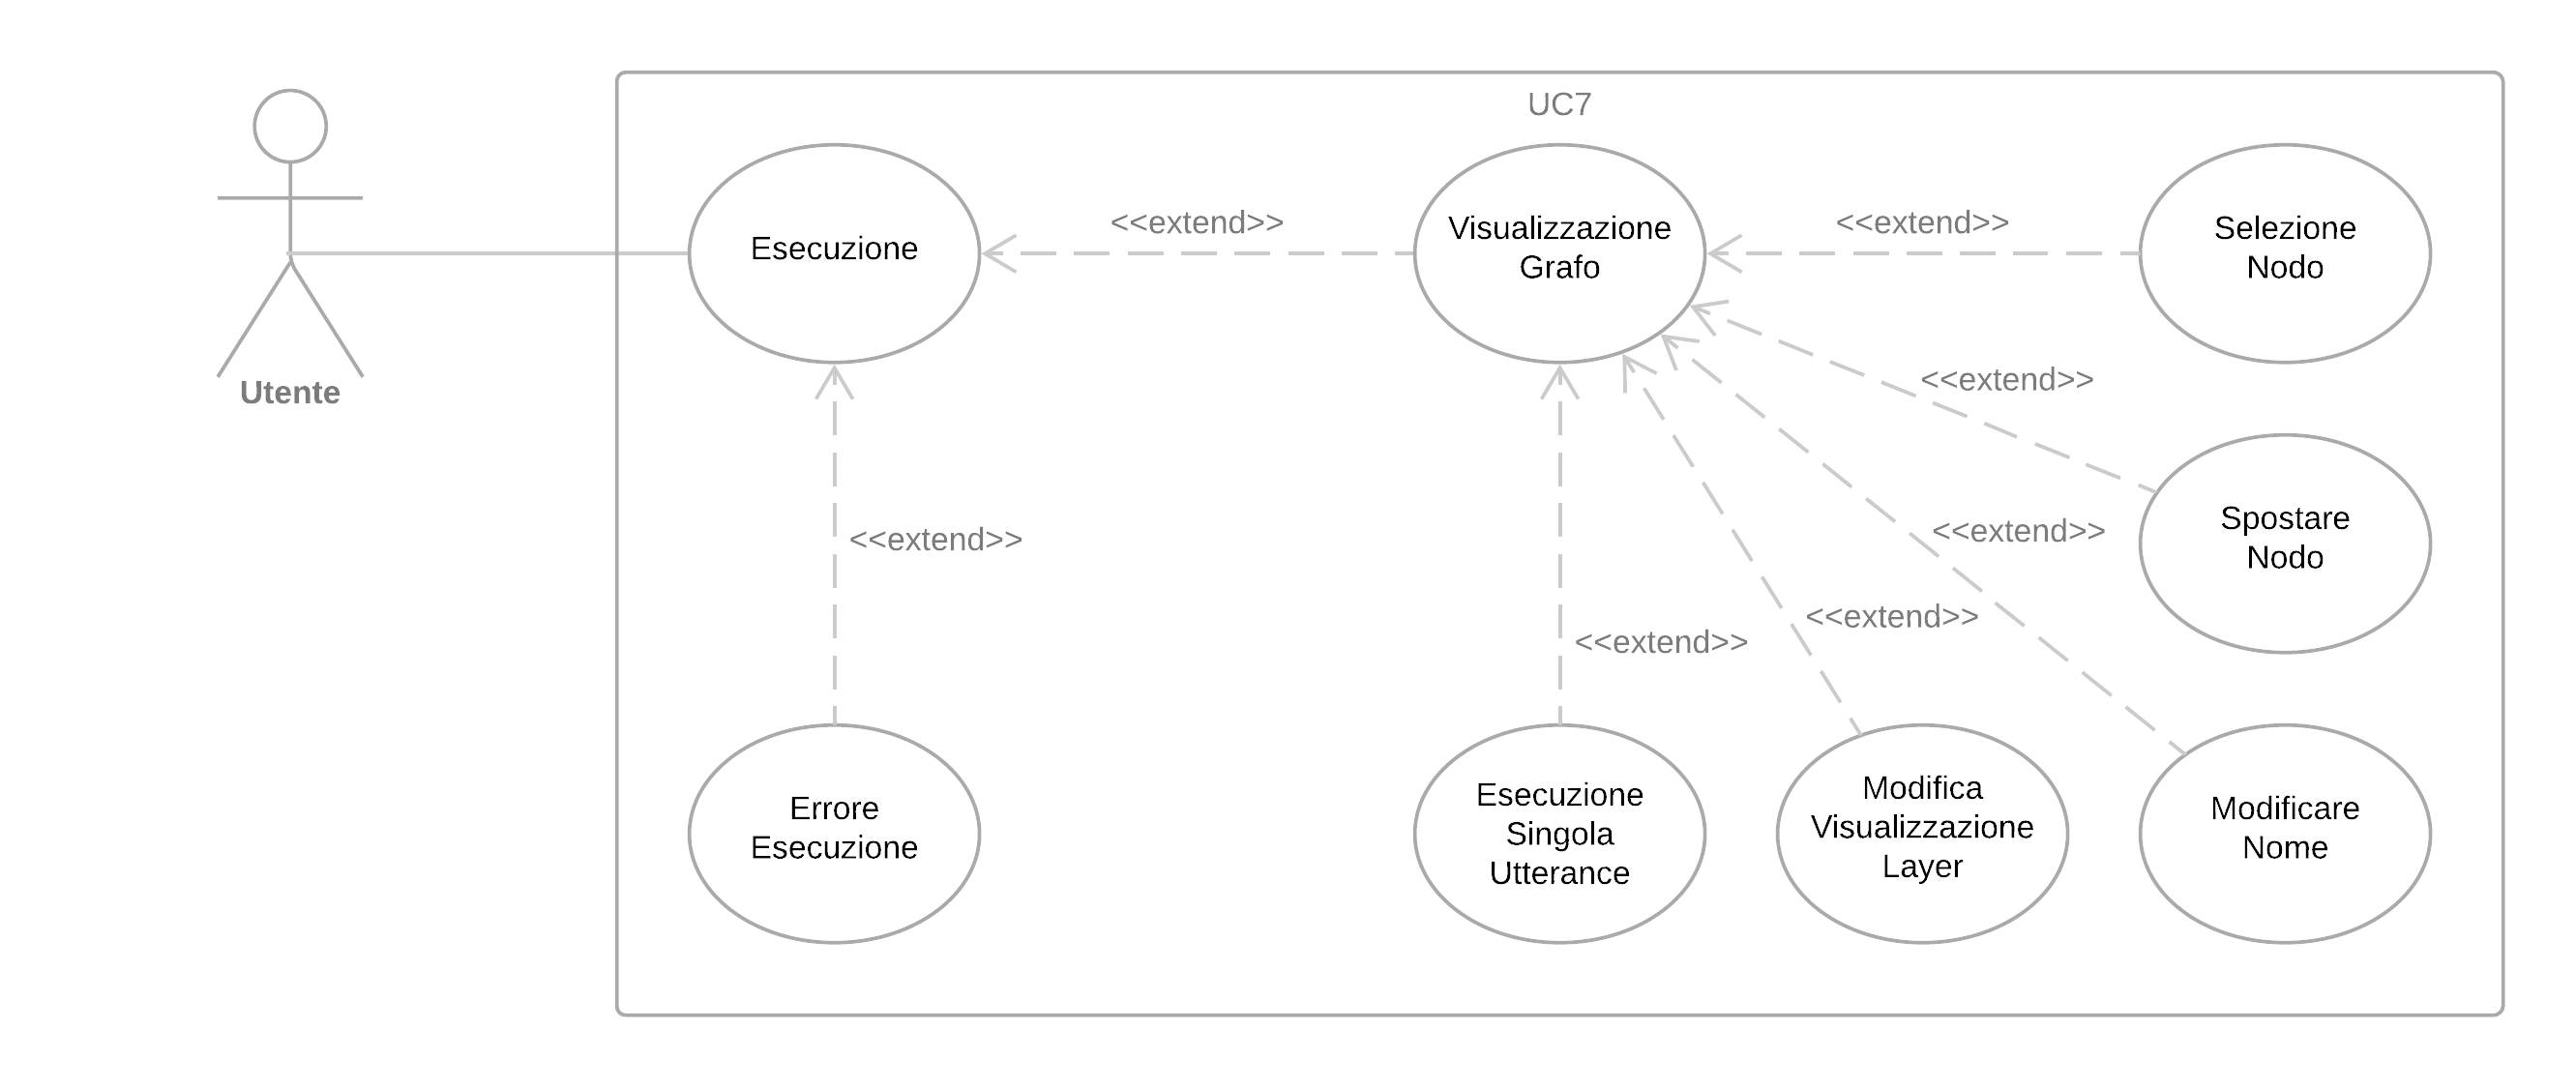
\includegraphics[width=\textwidth]{../img/UC07.png}
\end{figure}
\UserCase
{UC7}
{Utente}
{Non previsto}
{L'attore vuole eseguire Speect}
{Il file JSon è stato caricato correttamente}
{Speect elabora il testo selezionato e viene visualizzato il grafo}
{\begin{itemize}
		\item{} L'attore seleziona l'utterance type
		\item{} L'attore può compilare il campo di testo
		\item{} L'attore preme sul tasto di esecuzione
		\item{} Se il campo di testo è vuoto viene utilizzato il grafo come dato per l'utterance
		\item{} Vengono eseguiti gli utterance processor designati dall' utterance type
		\item{} Viene mostrato il grafo risultante dall'esecuzione \refer{UC7.2}
	\end{itemize}
}
{L'attore visualizza un messaggio di errore \refer{UC7.1}}

\section{UC7.1:Errore Esecuzione}
\UserCase
{UC7.1}
{Utente}
{Non previsto}
{L'attore visualizza a schermo l'errore di esecuzione di Speect }
{Speect ha fallito a eseguire la utterance e ha ritornato un errore}
{Viene visualizzato un messaggio di errore all'attore}
{Avvenimento dell'errore in fase di esecuzione}
{Non previsti}
\section{UC7.2:Visualizzazione Grafo}
\UserCase
{UC7.2}
{Utente}
{Non previsto}
{L'attore visualizza il grafo}
{Speect ha terminato l'esecuzione con successo}
{Viene visualizzato a schermo un grafo corretto con almeno un nodo cliccabile}
{
	\begin{itemize}
		\item{} L'attore può selezionare un nodo \refer{UC7.2.1}
		\item{} L'attore può spostare un nodo \refer{UC7.2.2}
	\end{itemize}
}
{Non previsti}

\section{UC7.2.1:Selezione Nodo}
\UserCase
{UC7.2.1}
{Utente}
{Non previsto}
{L'attore vuole selezionare un nodo per visualizzarne i dettagli}
{Un grafo con almeno un nodo è mostrato a schermo}
{Viene evidenziato il nodo del grafo e vengono mostrate le sue informazioni nella finestra apposita}
{
	\begin{itemize}
		\item{} L'attore clicca una volta sul nodo
		\item{} Il nodo viene evidenziato con un contorno giallo
		\item{} Nel riquadro apposito \ref{fig:GUI} vengono visualizzati i dati del grafo:
		\begin{enumerate}
			\item{} Name
			\item{} Part of Speech
		\end{enumerate}
		\item{} L'attore può modificare il name del nodo selezionato \refer{UC7.2.1.1}
		\item{} L'attore può modificare il PoS del nodo selezionato \refer{UC7.2.1.2} 
	\end{itemize}
}
{Non previsti}

\section{UC7.2.1.1:Modificare Name}
\UserCase
{UC7.2.1.1}
{Utente}
{Non previsto}
{L'attore vuole modificare il name del nodo selezionato}
{L'attore ha cliccato su un nodo \refer{UC7.2.1}}
{Il nodo cambia name}
{
	\begin{itemize}
		\item{} L'attore seleziona la casella di testo del name
		\item{} L'attore cancella il name precedente
		\item{} L'attore rimuove il focus dalla casella di testo
		\item{} Il name viene aggiornato
		\item{} Il grafo viene aggiornato \refer{UC7}
		\item{} Il grafo viene ristampato a schermo \refer{UC7.2}
	\end{itemize}
}
{Non previsti}

\section{UC7.2.1.2:Modificare PoS}
\UserCase
{UC7.2.1.2}
{Utente}
{Non previsto}
{L'attore vuole modificare il PoS del nodo selezionato}
{L'attore ha cliccato su un nodo \refer{UC7.2.1}}
{Il nodo cambia PoS}
{
	\begin{itemize}
		\item{} L'attore seleziona la casella di testo del PoS
		\item{} L'attore cancella il PoS precedente
		\item{} L'attore rimuove il focus dalla casella di testo
		\item{} Il PoS viene aggiornato
		\item{} Il grafo viene aggiornato \refer{UC7}
		\item{} Il grafo viene ristampato a schermo \refer{UC7.2}
	\end{itemize}
}
{Non previsti}

\section{UC7.2.2:Spostare Nodo}
\UserCase
{UC7.2.2}
{Utente}
{Non previsto}
{L'attore vuole spostare graficamente un nodo}
{Un grafo con almeno un nodo è mostrato a schermo}
{Il nodo viene spostato}
{
	\begin{itemize}
		\item{} L'attore trascina il nodo cliccando senza rilasciare
		\item{} Il nodo si sposta
		\item{} L'attore rilascia il click
		\item{} Il nodo rimane nella nuova posizione
	\end{itemize}
}
{Non previsti}

\section{UC7.2.3:Modifica Visualizzazione Relazione}
\UserCase
{UC7.2.3}
{Utente}
{Non previsto}
{L'attore vuole filtrare le relazioni del grafico}
{Un utterance type è stato scelto \refer{UC6}}
{Vengono mostrati tutti i layer di relazione selezionati}
{
	\begin{itemize}
		\item{} L'attore deseleziona una select box adiacente ad una relazione
		\item{} La relazione rimossa viene nascosta
	\end{itemize}
}
{Non previsti}
\section{UC7.2.4:Esecuzione Singola Utterance}
\UserCase
{UC7.2.4}
{Utente}
{Non previsto}
{L'attore vuole eseguire una singola utterance}
{Un utterance type è stato scelto \refer{UC6} }
{Viene eseguita l'utterance partendo dal grafo già presente o dal campo di testo scritto}
{
	\begin{itemize}
				\item{} L'attore seleziona l'utterance processor
		\item{} L'attore può compilare il campo di testo
		\item{} L'attore preme sul tasto di esecuzione adiacente all'utterance da eseguire \refer{UC6}
	\end{itemize}
}
{Non previsti}

\section{UC8:Esportazione Stato del Grafo}
\begin{figure}[H]
	\caption{UC8}
	\centering
	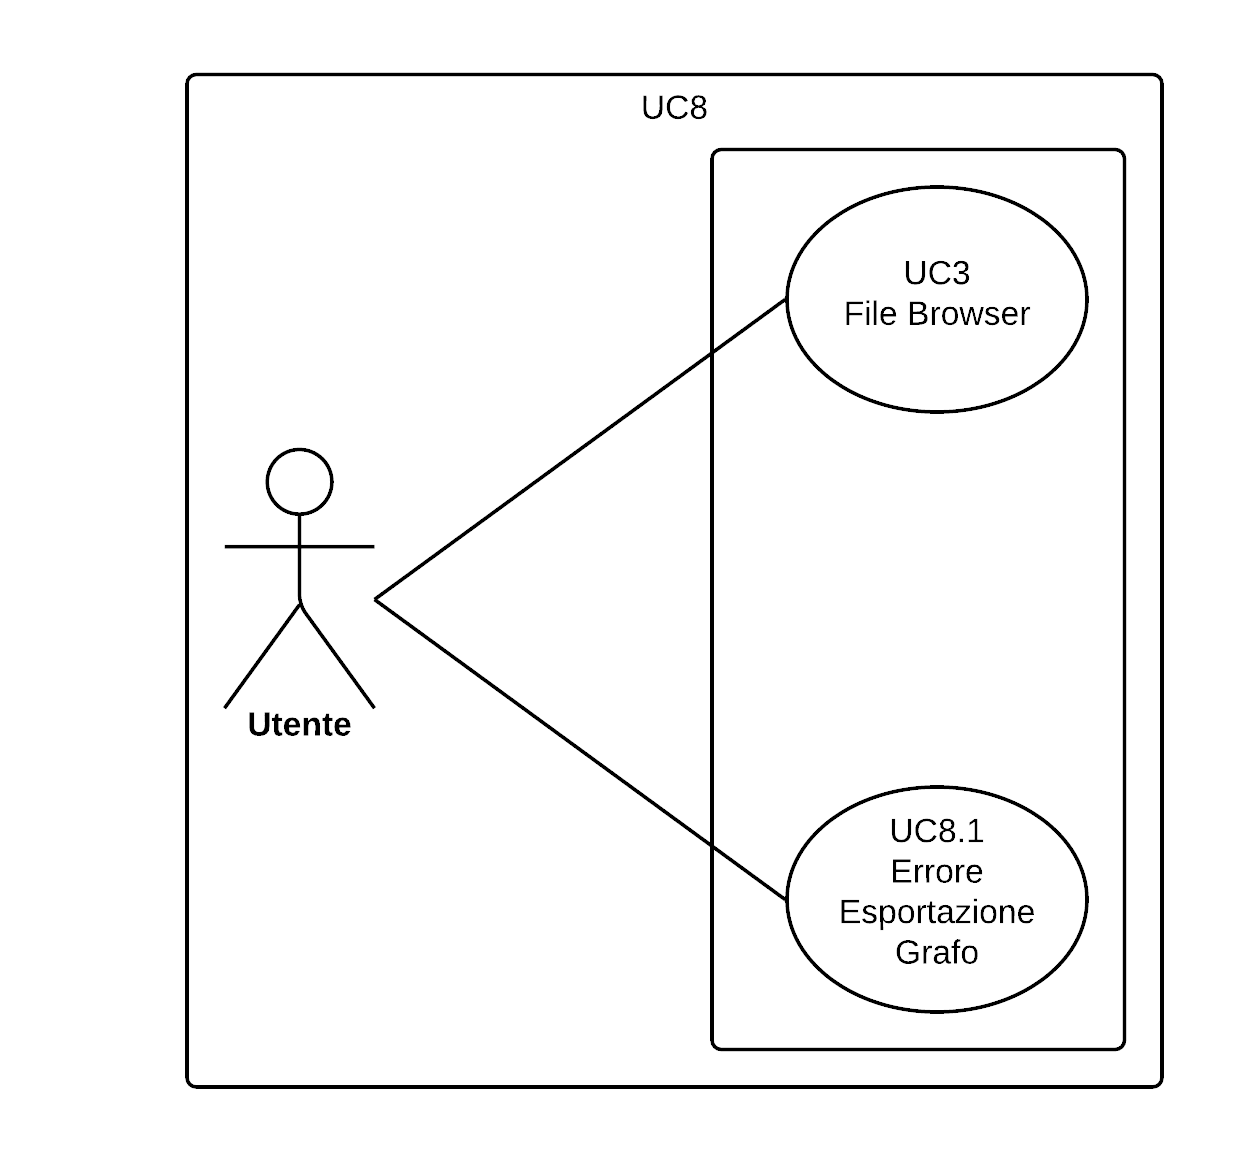
\includegraphics[width=\textwidth]{../img/UC08.png}
\end{figure}
\UserCase
{UC8}
{Utente}
{Non previsto}
{L'attore vuole esportare lo stato del grafo}
{Esiste un grafo esportabile}
{Il grafo viene esportato in file}
{
	\begin{itemize}
			\item{} Viene aperto il file browser
			\item{} L'attore seleziona il file da esportare
			\item{} L'attore preme su Salva Grafo
	\end{itemize}
}
{L'attore visualizza un messaggio di errore \refer{UC8.1}}

\section{UC8.1:Errore Esportazione Grafo}
\UserCase
{UC8.1}
{Utente}
{Non previsto}
{Avviene un errore durante l'esportazione}
{L'attore ha cercato di esportare un grafo}
{L'attore visualizza l'errore e nessuna operazione viene eseguita}
{Avvenimento dell'errore in fase di esportazione del grafo}
{Non previsti}

\section{UC9:Importazione Grafo}
\begin{figure}[H]
	\caption{UC9}
	\centering
	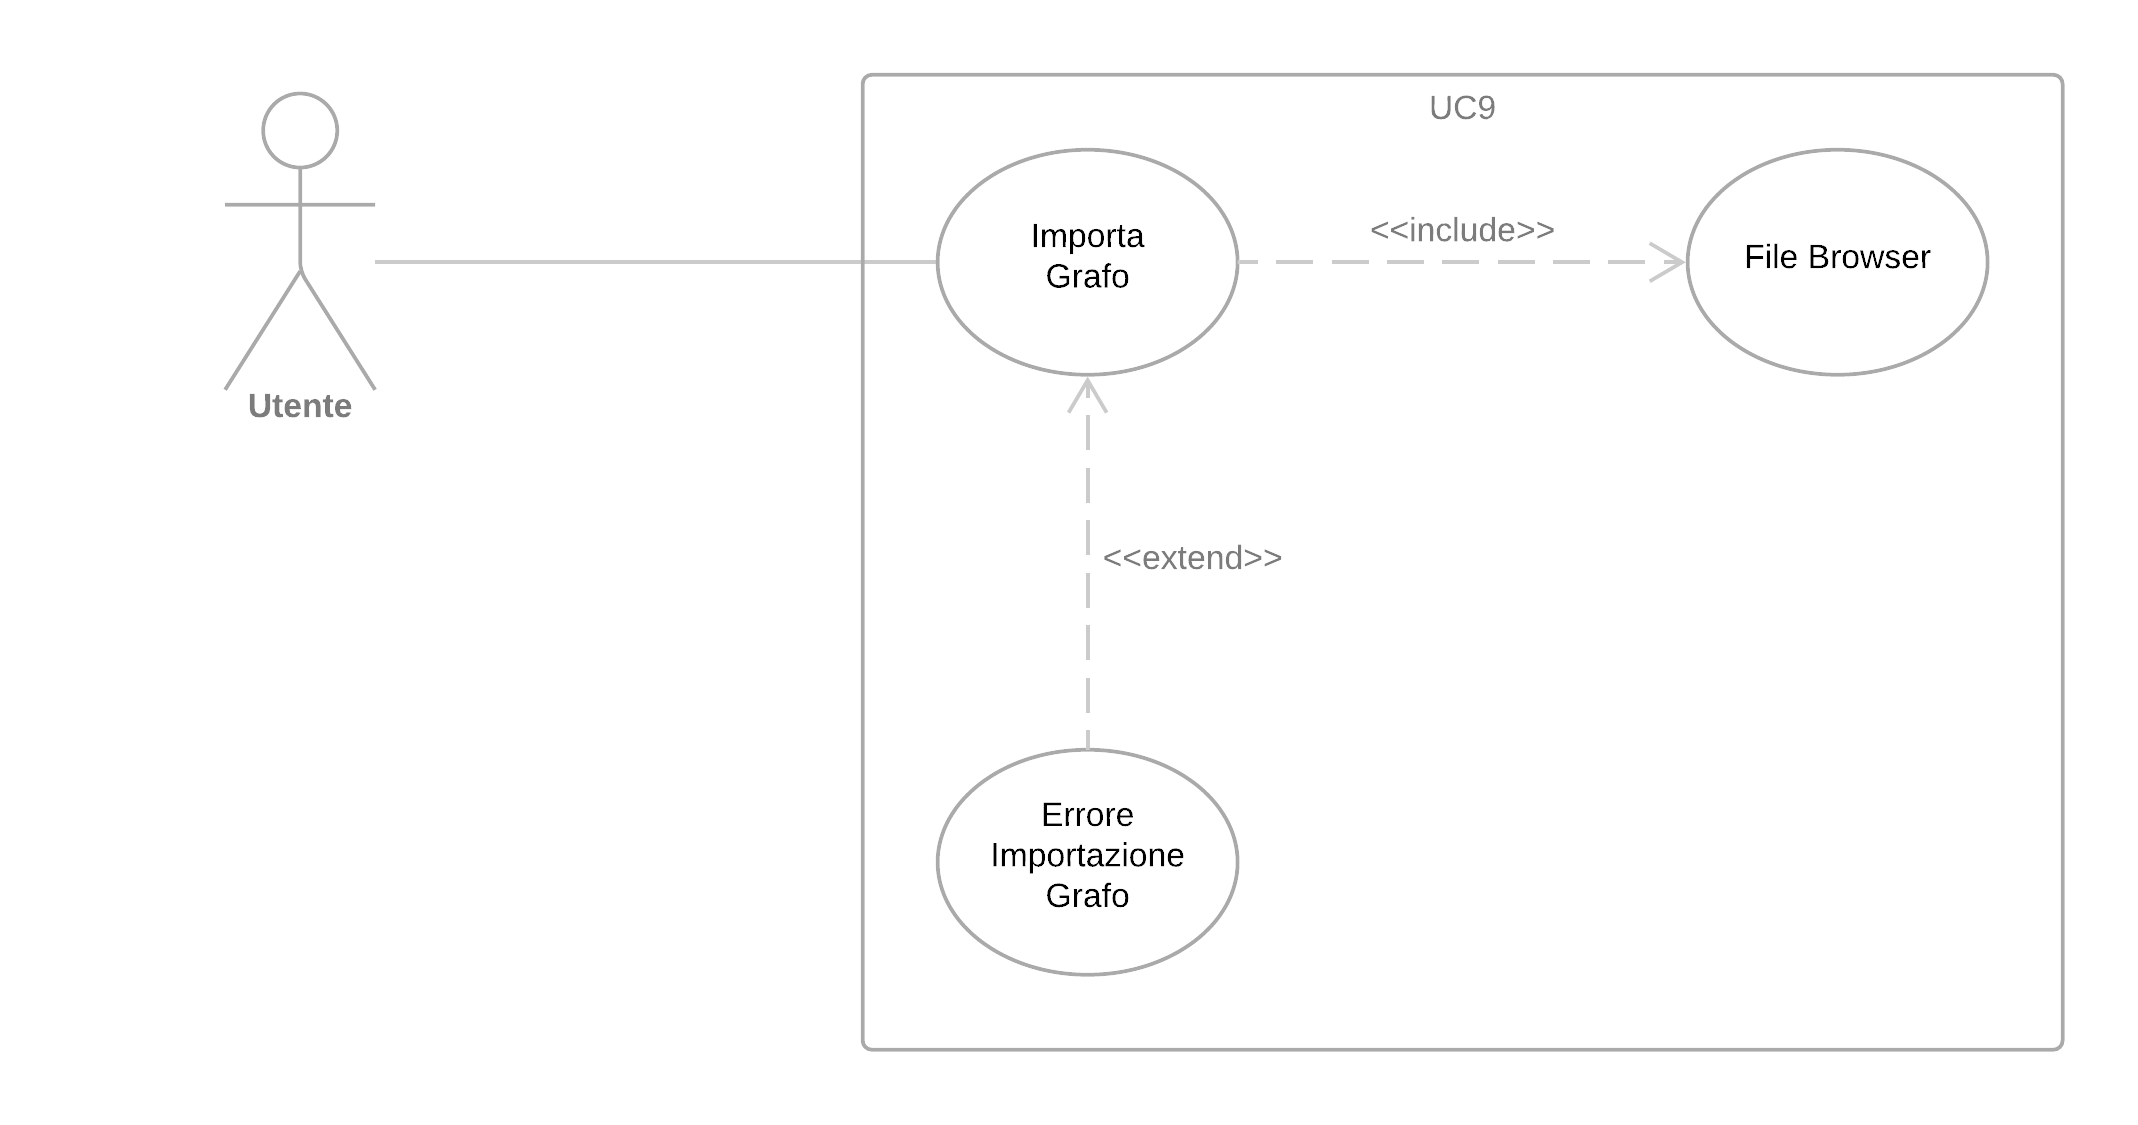
\includegraphics[width=\textwidth]{../img/UC09.png}
\end{figure}
\UserCase
{UC9}
{Utente}
{Non previsto}
{L'attore vuole importare lo stato del grafo}
{Esiste un grafo e l'attore ha cliccato Carica Grafo}
{Il grafo viene importato da file}
{
	\begin{itemize}
			\item{} Viene aperto il file browser
			\item{} L'attore seleziona il file da importare
			\item{} L'attore preme su Apri Grafo
	\end{itemize}
}
{L'attore visualizza un messaggio di errore \refer{UC9.1}}
\section{UC9.1:Errore Importazione Grafo}
\UserCase
{UC9.1}
{Utente}
{Non previsto}
{Avviene un errore durante l'importazione}
{L'attore ha cercato di importare un file scorretto}
{L'attore visualizza l'errore e nessuna operazione viene eseguita}
{Avvenimento dell'errore in fase di importazione del grafo}
{Non previsti}

\section{UC10:Ricerca Path}
\begin{figure}[H]
	\caption{UC10}
	\centering
	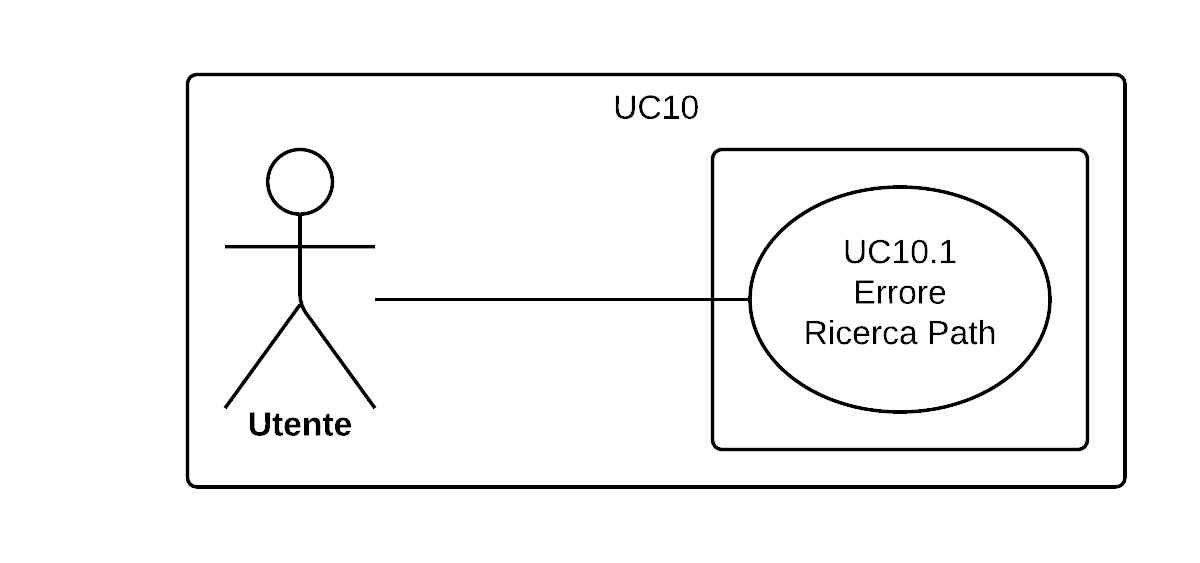
\includegraphics[width=\textwidth]{../img/UC10.png}
\end{figure}
\UserCase
{UC10}
{Utente}
{Non previsto}
{L'attore vuole cercare un percorso nel grafo}
{Esiste un grafo corretto, l'attore ha selezionato un nodo e premuto Ricerca Path nel menu}
{Se il path porta ad un nodo definito esso viene evidenziato \refer{UC7.2.1}}
{
	\begin{itemize}
		\item{} Viene visualizzata una finestra con una casella di testo e un pulsante
		\item{} L'attore inserisce il percorso da cercare
		\item{} L'attore preme il pulsante di Ricerca
		\item{} Se il percorso inizia dal nodo selezionato e finisce in un nodo esistente il nodo di arrivo viene evidenziato \refer{UC7.2.1}
 	\end{itemize}
}
{Viene visualizzato un errore \refer{UC10.1}}

\section{UC10.1:Errore Ricerca Path}
\UserCase
{UC10.1}
{Utente}
{Non previsto}
{L'attore vuole cercare un percorso nel grafo}
{Il percorso inserito dall'attore è sintatticamente errato e l'attore ha il pulsante di Ricerca}
{L'attore visualizza l'errore a schermo e si riapre la finestra di Ricerca \refer{UC10}}
{Avvenimento dell'errore in fase di ricerca}
{Non previsti}

\section{UC11:Salvataggio modifiche file JSon}
\begin{figure}[H]
	\caption{UC11}
	\centering
	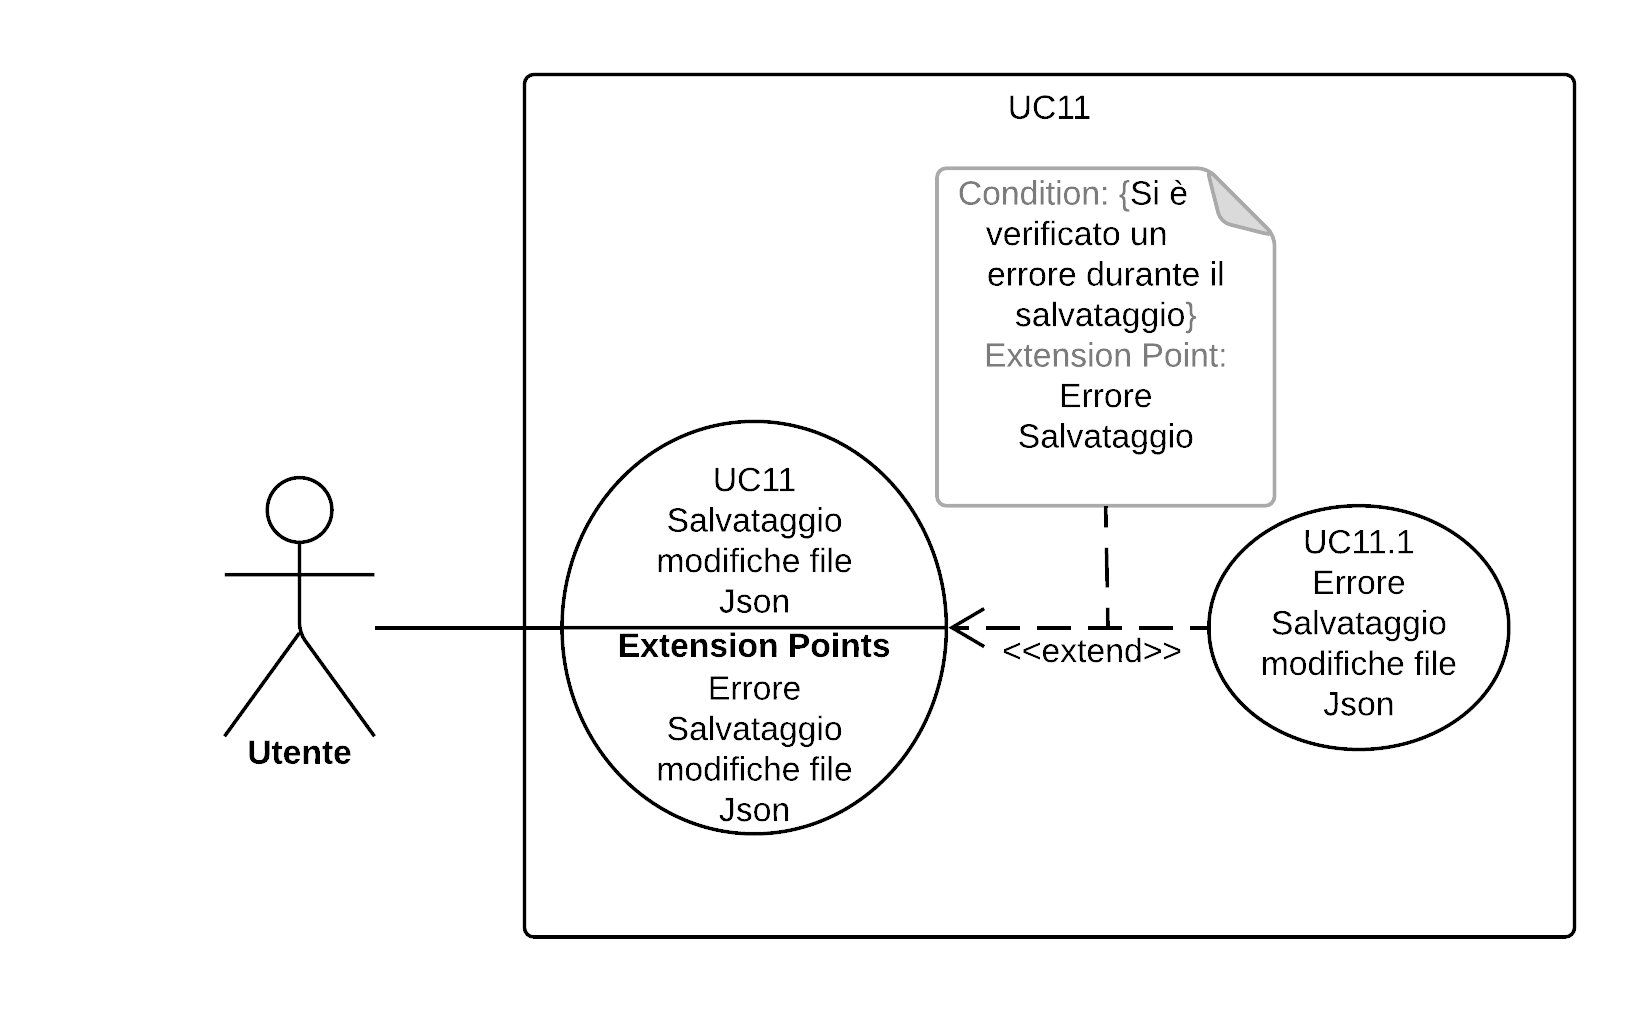
\includegraphics[width=\textwidth]{../img/UC11.png}
\end{figure}
\UserCase
{UC11}
{Utente}
{Non previsto}
{L'attore ha modificato gli Utterance Processor e vuole salvare il nuovo file JSon}
{Esiste un file Json correttamente aperto \refer{UC2} e l'attore ha modificato gli utterance processor \refer{UC6.1.1}}
{Le modifiche vengono Salvate}
{
	\begin{itemize}
		\item{} L'attore apre il menu file \refer{UC1}
		\item{} L'attore preme su Salva File JSon
	\end{itemize}
}
{Viene visualizzato un errore \refer{UC11.1}}
\section{UC11.1:Errore Salvataggio modifiche file JSon}
\UserCase
{UC11.1}
{Utente}
{Non previsto}
{L'attore ha provato a salvare il file JSon}
{L'operazione di salvataggio fallisce }
{L'attore visualizza la causa del fallimento e viene ripristinato lo stato precedente all'errore}
{Avvenimento dell'errore in fase di salvataggio}
{Non previsti}

\end{document}
